% 也可以弱化我们和ReAct框架
% 本质区别：operator、数据构造、RL training、description（可以提，不强调）

% （Flexible）现有工作需要人工成本，这些example很难提供。对于小白用户、表格很大，这一点是非常困难的，!!!举例...!!!
% 现有方法，operator是固定的，param也是固定的，搜索空间小很多；我们不需要用户给output

% Current Approaches Limitation - emphasizing orchestration failure

\section{Introduction}
\label{sec:intro}

% 加一下图例
%!TEX root = ../../main.tex
\begin{figure}[t]
    \centering 
    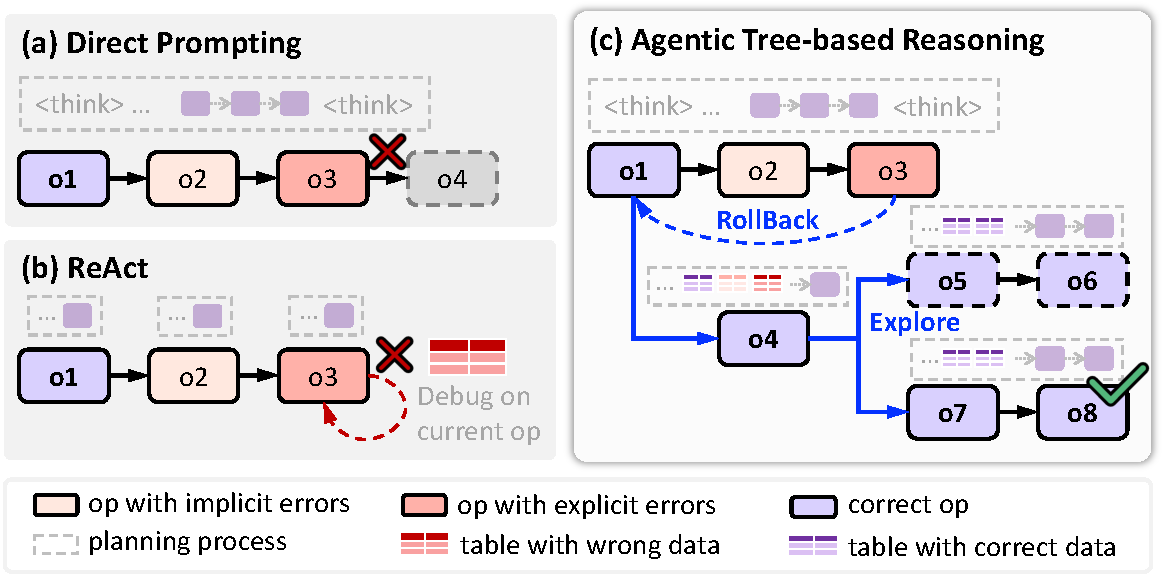
\includegraphics[width=0.99\columnwidth]{figures/fig/prompting_methods.pdf}
    % \vspace{-1em}
    \caption{Comparison of Different Inference Engine.
    }
    \label{fig:prompting_methods}
    % \vspace{-1em}
\end{figure}

%!TEX root = ../../main.tex
\begin{figure*}[!t]
    \centering 
    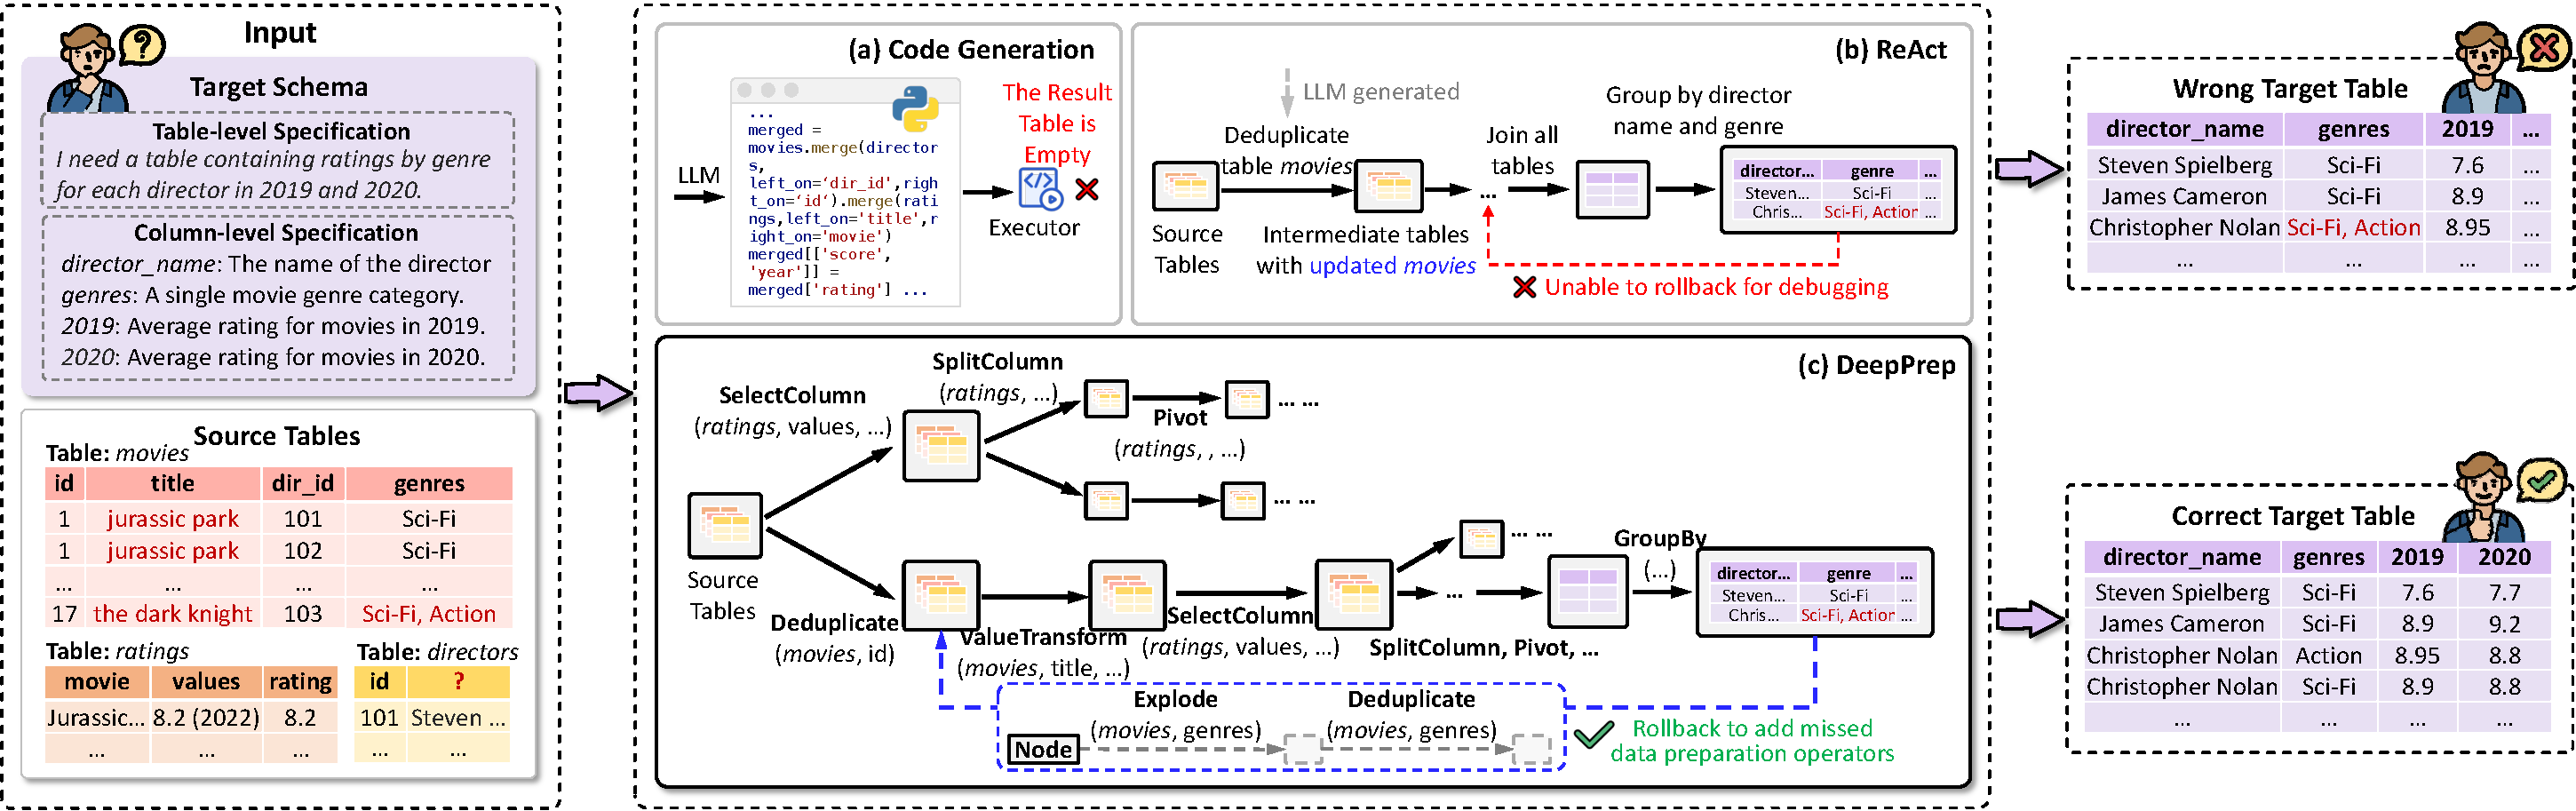
\includegraphics[width=0.95\textwidth]{figures/fig/introduction_example.pdf}
    \vspace{-1em}
    \caption{An illustrative example highlighting the core idea of \sys.
(a) Code generation makes decisions without grounding in intermediate execution results.
(b) ReAct-style approaches follow linear reasoning with limited ability to revise earlier decisions.
(c) \sys applies a tree-based structured exploration, which enables backtracking to resolve non-local errors.
    }
    \label{fig:introduction_example}
    \vspace{-1em}
\end{figure*}

\fmh{(High Level) Task: Table to table transformation with NL supervision. Make the reader convince that this is the naive and necessary process under the application scenerio.}

\fmh{Current Approaches Limitation. Fail to orchestrate the DP operations. Previous work (along with ReAct-based method) only focus on subtask. }

% Introduce DP
Data preparation (DP), encompassing column transformation, table reconstruction, and data cleaning, is fundamental to modern Business Intelligence (BI), Extract-Transform-Load (ETL), and analytics workflows.
% Motivate
In practical scenarios, data practitioners face the challenge of transforming heterogeneous raw tables into analysis-ready formats based on business requirements. 
% NL2DP is needed
Natural language (NL) guided table-to-table transformation represents the most intuitive and necessary paradigm for this task, as it eliminates the need for users to manually specify exact output schemas or write complex transformation scripts.
% An example to illusrate why the NL is needed, and the target table is hard to get.
This is particularly critical for non-technical users—business analysts, domain experts, and data scientists—who understand their data requirements but lack the expertise to implement complex multi-step transformations.
For instance, ...

% Current Approaches Limitation: emphasizing orchestration failure
\stitle{Current Approaches and Their Limitations.}
% Previous work only focus on subtask
The state-of-the-art (SOTA) results in DP are achieved through task-specific deep learning methodologies~\cite{DBLP:journals/pvldb/LiYLFT25, DBLP:conf/icde/FanHFC00024, yang2021auto}, which focus on isolated sub-problems rather than orchestrating multiple DP operations in unified end-to-end scenarios.
% Can not utilize NL as supervision
More critically, these methods require paired input-output table examples for training, where users must provide the exact target table structure—a requirement that is prohibitively difficult for large-scale tables with hundreds of columns and complex schemas.

% Why ReAct fails
Even the intuitive LLM-based ReAct prompting framework, which has shown promise in other domains, fundamentally fails in complex DP operation orchestration.
% An example of why ReAct fails
As illustrated in Figure~\ref{fig:introduction_example},...
This failure stems from the greedy, single-path nature of ReAct that lacks the ability to explore the vast combinatorial space of operator sequences.

\stitle{Key Distinctions from Existing Methods.} Our approach fundamentally differs from both traditional DP methods and ReAct-based frameworks in four critical aspects:

\etitle{(1) Flexible Operator Space with Dynamic Parameters.} Unlike existing methods with fixed operators and predetermined parameters, we define a comprehensive operator space (Table~\ref{tbl:operator_space}) covering 30+ operations, each with multiple configurable parameters. This creates an exponentially larger search space—with a 10-step workflow yielding over $10^{15}$ possible combinations when considering parameter variations—requiring sophisticated exploration strategies beyond greedy sequential reasoning.

\etitle{(2) No Ground Truth Output Requirements.} Current supervised methods require users to provide exact output tables, which is impractical for real-world scenarios. Consider a table with 1,000 rows and 50 columns requiring complex transformations—manually creating the desired output is error-prone and defeats the purpose of automation. Our approach only requires natural language descriptions, making DP accessible to non-technical users.

% Transition to our solution
\stitle{Unified End-to-End Data Preparation through Long-Chain Operation Orchestration.} To address these fundamental limitations, we propose a novel approach that enables end-to-end DP through natural language instructions alone, focusing on the critical challenge of orchestrating long sequences of DP operations.

\stitle{Technical Challenges.} Achieving unified NL-guided DP with long operation chains presents unique challenges:

% 1. 长链算子编排很难 --> 我们用数据构造方法给他提供这个能力
% 2. 
\etitle{(C1) Lack of Long-Chain Training Data.} Existing DP datasets only cover narrow sub-tasks with short operation sequences (typically 1-3 steps). Real-world DP scenarios, however, require long chains of 10+ operations with complex dependencies. For example, ...

\etitle{(C2) Exponential Search Space in Long-Chain Orchestration.} With our comprehensive operator set (Table~\ref{tbl:operator_space}), the search space grows exponentially with chain length. A 10-step workflow from 30 operators yields $30^{10} \approx 5.9 \times 10^{14}$ possible sequences before considering parameters. Current LLMs and ReAct-style frameworks fail to efficiently navigate this space, lacking mechanisms for parallel exploration, backtracking from failed paths, and maintaining coherence across long operation sequences.

\stitle{\sys: Tree-based Exploration for Long-Chain Data Preparation.} We propose \sys, featuring two key innovations to enable long-chain DP operation orchestration:

To address (C1), we introduce a \textbf{Long-Chain Data Construction} methodology that systematically generates verifiable training data with extended operation sequences. Starting from clean tables, we apply inverse operator chains of 10+ steps (introducing errors, inconsistencies, and structural issues in reverse order) to create complex dirty variants. Each synthetic example represents a complete DP workflow with clear dependencies between operations. Paired NL descriptions are generated to capture the high-level transformation goals without specifying exact outputs, ensuring both correctness and practical relevance.

To address (C2), we propose a Tree-based Exploration Framework enhanced by Curriculum-based Agentic Training paradigm. (1) Warmup SFT (Learn what operator do). (2) SFT on exploration data (Learn how to use tree-explore).  (3) RL training (Learn how to efficiently use tree-explore. 

\textbf{Trainable Tree-based Exploration Framework} that efficiently navigates the exponential space of long operation chains. Unlike ReAct's single-path approach, our framework: (1) generates multiple candidate operator sequences in parallel at each step, maintaining a tree of exploration paths; (2) executes candidates with immediate feedback, enabling informed backtracking when operations fail; and (3) employs reinforcement learning with carefully designed partial rewards that credit progress in long chains, even when the final output is not yet achieved. This multi-path exploration with execution feedback and intermediate rewards enables effective learning for long-horizon DP tasks.

\stitle{Contributions.} Our contributions are summarized as follows:

(1) We introduce a long-chain data construction methodology that generates verifiable DP workflows with 10+ operations and NL specifications, addressing the critical shortage of complex training data for operation orchestration (Section~\ref{sec:xxx}).

(2) We propose \sys, a trainable tree-based exploration framework with parallel search, execution feedback, and reinforcement learning optimization specifically designed for long-chain operation sequences, enabling efficient navigation of exponential operation spaces (Section~\ref{sec:xxx}).

(3) We demonstrate that \sys achieves state-of-the-art performance on both constructed long-chain benchmarks and existing DP tasks, improving end-to-end success rates by 47\% while reducing search costs by 63\% compared to ReAct-based approaches, particularly excelling on workflows requiring 10+ operations (Section~\ref{sec:xxx}).
